% Options for packages loaded elsewhere
\PassOptionsToPackage{unicode}{hyperref}
\PassOptionsToPackage{hyphens}{url}
%
\documentclass[
]{article}
\usepackage{amsmath,amssymb}
\usepackage{lmodern}
\usepackage{iftex}
\ifPDFTeX
  \usepackage[T1]{fontenc}
  \usepackage[utf8]{inputenc}
  \usepackage{textcomp} % provide euro and other symbols
\else % if luatex or xetex
  \usepackage{unicode-math}
  \defaultfontfeatures{Scale=MatchLowercase}
  \defaultfontfeatures[\rmfamily]{Ligatures=TeX,Scale=1}
\fi
% Use upquote if available, for straight quotes in verbatim environments
\IfFileExists{upquote.sty}{\usepackage{upquote}}{}
\IfFileExists{microtype.sty}{% use microtype if available
  \usepackage[]{microtype}
  \UseMicrotypeSet[protrusion]{basicmath} % disable protrusion for tt fonts
}{}
\makeatletter
\@ifundefined{KOMAClassName}{% if non-KOMA class
  \IfFileExists{parskip.sty}{%
    \usepackage{parskip}
  }{% else
    \setlength{\parindent}{0pt}
    \setlength{\parskip}{6pt plus 2pt minus 1pt}}
}{% if KOMA class
  \KOMAoptions{parskip=half}}
\makeatother
\usepackage{xcolor}
\IfFileExists{xurl.sty}{\usepackage{xurl}}{} % add URL line breaks if available
\IfFileExists{bookmark.sty}{\usepackage{bookmark}}{\usepackage{hyperref}}
\hypersetup{
  pdftitle={Homework 4},
  pdfauthor={PSTAT 131/231},
  hidelinks,
  pdfcreator={LaTeX via pandoc}}
\urlstyle{same} % disable monospaced font for URLs
\usepackage[margin=1in]{geometry}
\usepackage{color}
\usepackage{fancyvrb}
\newcommand{\VerbBar}{|}
\newcommand{\VERB}{\Verb[commandchars=\\\{\}]}
\DefineVerbatimEnvironment{Highlighting}{Verbatim}{commandchars=\\\{\}}
% Add ',fontsize=\small' for more characters per line
\usepackage{framed}
\definecolor{shadecolor}{RGB}{248,248,248}
\newenvironment{Shaded}{\begin{snugshade}}{\end{snugshade}}
\newcommand{\AlertTok}[1]{\textcolor[rgb]{0.94,0.16,0.16}{#1}}
\newcommand{\AnnotationTok}[1]{\textcolor[rgb]{0.56,0.35,0.01}{\textbf{\textit{#1}}}}
\newcommand{\AttributeTok}[1]{\textcolor[rgb]{0.77,0.63,0.00}{#1}}
\newcommand{\BaseNTok}[1]{\textcolor[rgb]{0.00,0.00,0.81}{#1}}
\newcommand{\BuiltInTok}[1]{#1}
\newcommand{\CharTok}[1]{\textcolor[rgb]{0.31,0.60,0.02}{#1}}
\newcommand{\CommentTok}[1]{\textcolor[rgb]{0.56,0.35,0.01}{\textit{#1}}}
\newcommand{\CommentVarTok}[1]{\textcolor[rgb]{0.56,0.35,0.01}{\textbf{\textit{#1}}}}
\newcommand{\ConstantTok}[1]{\textcolor[rgb]{0.00,0.00,0.00}{#1}}
\newcommand{\ControlFlowTok}[1]{\textcolor[rgb]{0.13,0.29,0.53}{\textbf{#1}}}
\newcommand{\DataTypeTok}[1]{\textcolor[rgb]{0.13,0.29,0.53}{#1}}
\newcommand{\DecValTok}[1]{\textcolor[rgb]{0.00,0.00,0.81}{#1}}
\newcommand{\DocumentationTok}[1]{\textcolor[rgb]{0.56,0.35,0.01}{\textbf{\textit{#1}}}}
\newcommand{\ErrorTok}[1]{\textcolor[rgb]{0.64,0.00,0.00}{\textbf{#1}}}
\newcommand{\ExtensionTok}[1]{#1}
\newcommand{\FloatTok}[1]{\textcolor[rgb]{0.00,0.00,0.81}{#1}}
\newcommand{\FunctionTok}[1]{\textcolor[rgb]{0.00,0.00,0.00}{#1}}
\newcommand{\ImportTok}[1]{#1}
\newcommand{\InformationTok}[1]{\textcolor[rgb]{0.56,0.35,0.01}{\textbf{\textit{#1}}}}
\newcommand{\KeywordTok}[1]{\textcolor[rgb]{0.13,0.29,0.53}{\textbf{#1}}}
\newcommand{\NormalTok}[1]{#1}
\newcommand{\OperatorTok}[1]{\textcolor[rgb]{0.81,0.36,0.00}{\textbf{#1}}}
\newcommand{\OtherTok}[1]{\textcolor[rgb]{0.56,0.35,0.01}{#1}}
\newcommand{\PreprocessorTok}[1]{\textcolor[rgb]{0.56,0.35,0.01}{\textit{#1}}}
\newcommand{\RegionMarkerTok}[1]{#1}
\newcommand{\SpecialCharTok}[1]{\textcolor[rgb]{0.00,0.00,0.00}{#1}}
\newcommand{\SpecialStringTok}[1]{\textcolor[rgb]{0.31,0.60,0.02}{#1}}
\newcommand{\StringTok}[1]{\textcolor[rgb]{0.31,0.60,0.02}{#1}}
\newcommand{\VariableTok}[1]{\textcolor[rgb]{0.00,0.00,0.00}{#1}}
\newcommand{\VerbatimStringTok}[1]{\textcolor[rgb]{0.31,0.60,0.02}{#1}}
\newcommand{\WarningTok}[1]{\textcolor[rgb]{0.56,0.35,0.01}{\textbf{\textit{#1}}}}
\usepackage{graphicx}
\makeatletter
\def\maxwidth{\ifdim\Gin@nat@width>\linewidth\linewidth\else\Gin@nat@width\fi}
\def\maxheight{\ifdim\Gin@nat@height>\textheight\textheight\else\Gin@nat@height\fi}
\makeatother
% Scale images if necessary, so that they will not overflow the page
% margins by default, and it is still possible to overwrite the defaults
% using explicit options in \includegraphics[width, height, ...]{}
\setkeys{Gin}{width=\maxwidth,height=\maxheight,keepaspectratio}
% Set default figure placement to htbp
\makeatletter
\def\fps@figure{htbp}
\makeatother
\setlength{\emergencystretch}{3em} % prevent overfull lines
\providecommand{\tightlist}{%
  \setlength{\itemsep}{0pt}\setlength{\parskip}{0pt}}
\setcounter{secnumdepth}{-\maxdimen} % remove section numbering
\ifLuaTeX
  \usepackage{selnolig}  % disable illegal ligatures
\fi

\title{Homework 4}
\author{PSTAT 131/231}
\date{}

\begin{document}
\maketitle

{
\setcounter{tocdepth}{2}
\tableofcontents
}
\hypertarget{resampling}{%
\subsection{Resampling}\label{resampling}}

For this assignment, we will continue working with part of a
\href{https://www.kaggle.com/c/titanic/overview}{Kaggle data set} that
was the subject of a machine learning competition and is often used for
practicing ML models. The goal is classification; specifically, to
predict which passengers would survive the
\href{https://en.wikipedia.org/wiki/Titanic}{Titanic shipwreck}.

\begin{figure}
\centering
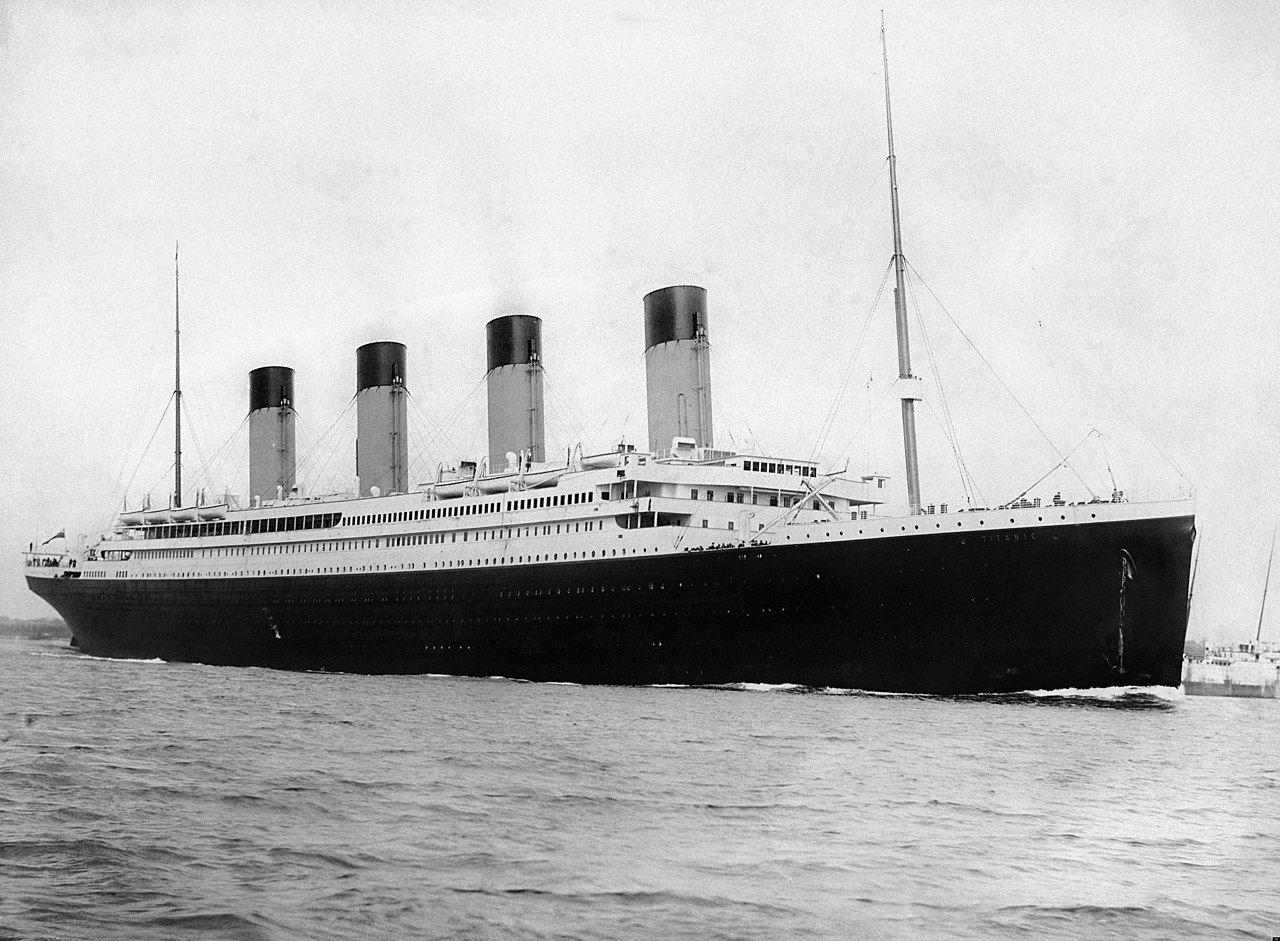
\includegraphics[width=3.78125in,height=\textheight]{images/RMS_Titanic.jpg}
\caption{Fig. 1: RMS Titanic departing Southampton on April 10, 1912.}
\end{figure}

Load the data from \texttt{data/titanic.csv} into \emph{R} and
familiarize yourself with the variables it contains using the codebook
(\texttt{data/titanic\_codebook.txt}).

Notice that \texttt{survived} and \texttt{pclass} should be changed to
factors. When changing \texttt{survived} to a factor, you may want to
reorder the factor so that \emph{``Yes''} is the first level.

Make sure you load the \texttt{tidyverse} and \texttt{tidymodels}!

\begin{Shaded}
\begin{Highlighting}[]
\FunctionTok{library}\NormalTok{(tidyverse)}
\FunctionTok{library}\NormalTok{(tidymodels)}
\FunctionTok{library}\NormalTok{(rlang)}
\FunctionTok{library}\NormalTok{(corrr)}
\FunctionTok{library}\NormalTok{(klaR)}
\FunctionTok{library}\NormalTok{(discrim)}
\FunctionTok{library}\NormalTok{(poissonreg)}

\CommentTok{\#library(ISLR) \# For the Smarket data set}
\CommentTok{\#library(ISLR2) \# For the Bikeshare data set}
\FunctionTok{tidymodels\_prefer}\NormalTok{()}

\FunctionTok{set.seed}\NormalTok{(}\DecValTok{22}\NormalTok{)}

\CommentTok{\# Load Data}
\NormalTok{rawData }\OtherTok{\textless{}{-}} \FunctionTok{read.csv}\NormalTok{(}\StringTok{"data/titanic.csv"}\NormalTok{)}
\FunctionTok{head}\NormalTok{(rawData)}
\end{Highlighting}
\end{Shaded}

\begin{verbatim}
##   passenger_id survived pclass
## 1            1       No      3
## 2            2      Yes      1
## 3            3      Yes      3
## 4            4      Yes      1
## 5            5       No      3
## 6            6       No      3
##                                                  name    sex age sib_sp parch
## 1                             Braund, Mr. Owen Harris   male  22      1     0
## 2 Cumings, Mrs. John Bradley (Florence Briggs Thayer) female  38      1     0
## 3                              Heikkinen, Miss. Laina female  26      0     0
## 4        Futrelle, Mrs. Jacques Heath (Lily May Peel) female  35      1     0
## 5                            Allen, Mr. William Henry   male  35      0     0
## 6                                    Moran, Mr. James   male  NA      0     0
##             ticket    fare cabin embarked
## 1        A/5 21171  7.2500  <NA>        S
## 2         PC 17599 71.2833   C85        C
## 3 STON/O2. 3101282  7.9250  <NA>        S
## 4           113803 53.1000  C123        S
## 5           373450  8.0500  <NA>        S
## 6           330877  8.4583  <NA>        Q
\end{verbatim}

\begin{Shaded}
\begin{Highlighting}[]
\CommentTok{\# Copy dataframe}
\NormalTok{data }\OtherTok{\textless{}{-}} \FunctionTok{duplicate}\NormalTok{(rawData, }\AttributeTok{shallow =} \ConstantTok{FALSE}\NormalTok{)}

\CommentTok{\#reorder factors}
\NormalTok{data}\SpecialCharTok{$}\NormalTok{survived }\OtherTok{\textless{}{-}} \FunctionTok{factor}\NormalTok{(data}\SpecialCharTok{$}\NormalTok{survived, }\AttributeTok{levels =} \FunctionTok{c}\NormalTok{(}\StringTok{"Yes"}\NormalTok{, }\StringTok{"No"}\NormalTok{))}
\NormalTok{data}\SpecialCharTok{$}\NormalTok{pclass }\OtherTok{\textless{}{-}} \FunctionTok{factor}\NormalTok{(data}\SpecialCharTok{$}\NormalTok{pclass)}
\CommentTok{\# data$sex \textless{}{-} factor(data$sex, levels = c("female", "male"))}

\FunctionTok{levels}\NormalTok{(data}\SpecialCharTok{$}\NormalTok{survived)}
\end{Highlighting}
\end{Shaded}

\begin{verbatim}
## [1] "Yes" "No"
\end{verbatim}

\begin{Shaded}
\begin{Highlighting}[]
\FunctionTok{levels}\NormalTok{(data}\SpecialCharTok{$}\NormalTok{pclass)}
\end{Highlighting}
\end{Shaded}

\begin{verbatim}
## [1] "1" "2" "3"
\end{verbatim}

\emph{Remember that you'll need to set a seed at the beginning of the
document to reproduce your results.}

Create a recipe for this dataset \textbf{identical} to the recipe you
used in Homework 3.

\hypertarget{question-1}{%
\subsubsection{Question 1}\label{question-1}}

Split the data, stratifying on the outcome variable, \texttt{survived.}
You should choose the proportions to split the data into. Verify that
the training and testing data sets have the appropriate number of
observations.

\begin{Shaded}
\begin{Highlighting}[]
\NormalTok{titanicSplit }\OtherTok{\textless{}{-}} \FunctionTok{initial\_split}\NormalTok{(data, }
                              \AttributeTok{prop =} \FloatTok{0.8}\NormalTok{, }
                              \AttributeTok{strata =}\NormalTok{ survived)}

\NormalTok{dataTrain }\OtherTok{\textless{}{-}} \FunctionTok{training}\NormalTok{(titanicSplit)}
\NormalTok{dataTest }\OtherTok{\textless{}{-}} \FunctionTok{testing}\NormalTok{(titanicSplit)}

\NormalTok{titanicSplit}
\end{Highlighting}
\end{Shaded}

\begin{verbatim}
## <Analysis/Assess/Total>
## <712/179/891>
\end{verbatim}

\begin{Shaded}
\begin{Highlighting}[]
\FunctionTok{names}\NormalTok{(dataTrain)}
\end{Highlighting}
\end{Shaded}

\begin{verbatim}
##  [1] "passenger_id" "survived"     "pclass"       "name"         "sex"         
##  [6] "age"          "sib_sp"       "parch"        "ticket"       "fare"        
## [11] "cabin"        "embarked"
\end{verbatim}

\begin{Shaded}
\begin{Highlighting}[]
\NormalTok{lm\_spec }\OtherTok{\textless{}{-}} \FunctionTok{linear\_reg}\NormalTok{() }\SpecialCharTok{\%\textgreater{}\%}
  \FunctionTok{set\_mode}\NormalTok{(}\StringTok{"regression"}\NormalTok{) }\SpecialCharTok{\%\textgreater{}\%}
  \FunctionTok{set\_engine}\NormalTok{(}\StringTok{"lm"}\NormalTok{)}


\CommentTok{\# titanicPolyTunedRecipe \textless{}{-} recipe(survived \textasciitilde{} pclass +}
\CommentTok{\#                            sex +}
\CommentTok{\#                            age +}
\CommentTok{\#                            sib\_sp +}
\CommentTok{\#                            parch +}
\CommentTok{\#                            fare, data = dataTrain) \%\textgreater{}\%}
\CommentTok{\#     step\_impute\_linear(age) \%\textgreater{}\%}
\CommentTok{\#     step\_dummy(all\_nominal\_predictors()) \%\textgreater{}\%}
\CommentTok{\#     step\_interact(terms = \textasciitilde{} sex\_male:fare) \%\textgreater{}\%}
\CommentTok{\#     step\_interact(terms = \textasciitilde{} age:fare) \%\textgreater{}\%}
\CommentTok{\#     step\_poly(survived, degree = tune())}


\CommentTok{\# poly\_tuned\_wf \textless{}{-} workflow() \%\textgreater{}\%}
\CommentTok{\#   add\_recipe(titanicPolyTunedRecipe) \%\textgreater{}\%}
\CommentTok{\#   add\_model(lm\_spec)}



\CommentTok{\# {-}{-}{-}{-}{-}{-}{-}{-}{-}{-}{-}{-}{-}{-}{-}{-}{-}{-}{-}{-}{-}{-}{-}{-}{-}\# {-}{-}{-}{-}{-}{-}{-}{-}{-}{-}{-}{-}{-}{-}{-}{-}{-}{-}{-}{-}{-}{-}{-}{-}{-}\# {-}{-}{-}{-}{-}{-}{-}{-}{-}{-}{-}{-}{-}{-}{-}{-}{-}{-}{-}{-}{-}{-}{-}{-}{-}}


\NormalTok{titanicRecipe }\OtherTok{\textless{}{-}} \FunctionTok{recipe}\NormalTok{(survived }\SpecialCharTok{\textasciitilde{}}\NormalTok{ pclass }\SpecialCharTok{+} 
\NormalTok{                           sex }\SpecialCharTok{+} 
\NormalTok{                           age }\SpecialCharTok{+} 
\NormalTok{                           sib\_sp }\SpecialCharTok{+}  
\NormalTok{                           parch }\SpecialCharTok{+}
\NormalTok{                           fare, }\AttributeTok{data =}\NormalTok{ dataTrain) }\SpecialCharTok{\%\textgreater{}\%}
     \FunctionTok{step\_impute\_linear}\NormalTok{(age) }\SpecialCharTok{\%\textgreater{}\%}
     \FunctionTok{step\_dummy}\NormalTok{(}\FunctionTok{all\_nominal\_predictors}\NormalTok{()) }\SpecialCharTok{\%\textgreater{}\%}
     \FunctionTok{step\_interact}\NormalTok{(}\AttributeTok{terms =} \SpecialCharTok{\textasciitilde{}} \FunctionTok{starts\_with}\NormalTok{(}\StringTok{"sex"}\NormalTok{)}\SpecialCharTok{:}\NormalTok{fare) }\SpecialCharTok{\%\textgreater{}\%}
     \FunctionTok{step\_interact}\NormalTok{(}\AttributeTok{terms =} \SpecialCharTok{\textasciitilde{}}\NormalTok{ age}\SpecialCharTok{:}\NormalTok{fare)}


\NormalTok{titanicWkflw }\OtherTok{\textless{}{-}} \FunctionTok{workflow}\NormalTok{() }\SpecialCharTok{\%\textgreater{}\%}
  \FunctionTok{add\_model}\NormalTok{(lm\_spec) }\SpecialCharTok{\%\textgreater{}\%}
  \FunctionTok{add\_recipe}\NormalTok{(titanicRecipe)}
\end{Highlighting}
\end{Shaded}

\begin{Shaded}
\begin{Highlighting}[]
\CommentTok{\# fit(poly\_tuned\_wf, data = dataTrain)}
\CommentTok{\#fit(titanicWkflw, data = dataTrain)}
\end{Highlighting}
\end{Shaded}

\hypertarget{question-2}{%
\subsubsection{Question 2}\label{question-2}}

Fold the \textbf{training} data. Use \emph{k}-fold cross-validation,
with \(k = 10\).

\begin{Shaded}
\begin{Highlighting}[]
\CommentTok{\# titanicPolyTunedRecipe \textless{}{-} titanicRecipe \%\textgreater{}\%}
\CommentTok{\#   step\_poly(survived, degree = tune())}
\CommentTok{\# }
\CommentTok{\# poly\_tuned\_wf \textless{}{-} workflow() \%\textgreater{}\%}
\CommentTok{\#   add\_recipe(titanicPolyTunedRecipe) \%\textgreater{}\%}
\CommentTok{\#   add\_model(lm\_spec)}

\NormalTok{titanicFolds }\OtherTok{\textless{}{-}} \FunctionTok{vfold\_cv}\NormalTok{(dataTrain, }\AttributeTok{v =} \DecValTok{10}\NormalTok{)}
\NormalTok{titanicFolds}
\end{Highlighting}
\end{Shaded}

\begin{verbatim}
## #  10-fold cross-validation 
## # A tibble: 10 x 2
##    splits           id    
##    <list>           <chr> 
##  1 <split [640/72]> Fold01
##  2 <split [640/72]> Fold02
##  3 <split [641/71]> Fold03
##  4 <split [641/71]> Fold04
##  5 <split [641/71]> Fold05
##  6 <split [641/71]> Fold06
##  7 <split [641/71]> Fold07
##  8 <split [641/71]> Fold08
##  9 <split [641/71]> Fold09
## 10 <split [641/71]> Fold10
\end{verbatim}

\begin{Shaded}
\begin{Highlighting}[]
\NormalTok{degree\_grid }\OtherTok{\textless{}{-}} \FunctionTok{grid\_regular}\NormalTok{(}\FunctionTok{degree}\NormalTok{(}\AttributeTok{range =} \FunctionTok{c}\NormalTok{(}\DecValTok{1}\NormalTok{,}\DecValTok{10}\NormalTok{)), }\AttributeTok{levels =} \DecValTok{10}\NormalTok{)}
\NormalTok{degree\_grid}
\end{Highlighting}
\end{Shaded}

\begin{verbatim}
## # A tibble: 10 x 1
##    degree
##     <dbl>
##  1      1
##  2      2
##  3      3
##  4      4
##  5      5
##  6      6
##  7      7
##  8      8
##  9      9
## 10     10
\end{verbatim}

\begin{Shaded}
\begin{Highlighting}[]
\CommentTok{\# tune\_res \textless{}{-} tune\_grid(}
\CommentTok{\#   object = poly\_tuned\_wf,}
\CommentTok{\#   resamples = titanicFolds,}
\CommentTok{\#   grid = degree\_grid,}
\CommentTok{\#   control = control\_grid(verbose = TRUE)}
\CommentTok{\# )}
\end{Highlighting}
\end{Shaded}

\hypertarget{question-3}{%
\subsubsection{Question 3}\label{question-3}}

In your own words, explain what we are doing in Question 2. What is
\emph{k}-fold cross-validation? Why should we use it, rather than simply
fitting and testing models on the entire training set? If we
\textbf{did} use the entire training set, what resampling method would
that be?

\textbf{In question 2, we are taking the training data and dividing it
into 10 groups. Then for each group, we train a model on the remainder
of the data, and use the group as testing data. In this way we train 10
different models on various subsets of the same dataset. We can then
test the effectiveness of each model and select that which the most
effective. We use k folds cross validation in order to find a model that
have a smaller bias. Using a simple test/train split method may result
in a biased model, if the data happens to be split unevenly. If we did
use the entire training dataset, the resampling method would be that of
simple train/test split validation}

\hypertarget{question-4}{%
\subsubsection{Question 4}\label{question-4}}

Set up workflows for 3 models:

\begin{enumerate}
\def\labelenumi{\arabic{enumi}.}
\tightlist
\item
  A logistic regression with the \texttt{glm} engine;
\item
  A linear discriminant analysis with the \texttt{MASS} engine;
\item
  A quadratic discriminant analysis with the \texttt{MASS} engine.
\end{enumerate}

How many models, total, across all folds, will you be fitting to the
data? To answer, think about how many folds there are, and how many
models you'll fit to each fold.

There are 10 folds and 3 models, so across all folds, we fit 30 models
to the data.

\begin{Shaded}
\begin{Highlighting}[]
\NormalTok{logReg }\OtherTok{\textless{}{-}} \FunctionTok{logistic\_reg}\NormalTok{() }\SpecialCharTok{\%\textgreater{}\%}
  \FunctionTok{set\_mode}\NormalTok{(}\StringTok{"classification"}\NormalTok{) }\SpecialCharTok{\%\textgreater{}\%}
  \FunctionTok{set\_engine}\NormalTok{(}\StringTok{"glm"}\NormalTok{)}

\NormalTok{logWkflw }\OtherTok{\textless{}{-}} \FunctionTok{workflow}\NormalTok{() }\SpecialCharTok{\%\textgreater{}\%}
  \FunctionTok{add\_model}\NormalTok{(logReg) }\SpecialCharTok{\%\textgreater{}\%}
  \FunctionTok{add\_recipe}\NormalTok{(titanicRecipe)}



\NormalTok{ldaMod }\OtherTok{\textless{}{-}} \FunctionTok{discrim\_linear}\NormalTok{() }\SpecialCharTok{\%\textgreater{}\%}
  \FunctionTok{set\_mode}\NormalTok{(}\StringTok{"classification"}\NormalTok{) }\SpecialCharTok{\%\textgreater{}\%}
  \FunctionTok{set\_engine}\NormalTok{(}\StringTok{"MASS"}\NormalTok{)}

\NormalTok{ldaWkflw }\OtherTok{\textless{}{-}} \FunctionTok{workflow}\NormalTok{() }\SpecialCharTok{\%\textgreater{}\%}
  \FunctionTok{add\_model}\NormalTok{(ldaMod) }\SpecialCharTok{\%\textgreater{}\%}
  \FunctionTok{add\_recipe}\NormalTok{(titanicRecipe)}
  


\NormalTok{qdaMod }\OtherTok{\textless{}{-}} \FunctionTok{discrim\_quad}\NormalTok{() }\SpecialCharTok{\%\textgreater{}\%}
  \FunctionTok{set\_mode}\NormalTok{(}\StringTok{"classification"}\NormalTok{) }\SpecialCharTok{\%\textgreater{}\%}
  \FunctionTok{set\_engine}\NormalTok{(}\StringTok{"MASS"}\NormalTok{)}

\NormalTok{qdaWkflw }\OtherTok{\textless{}{-}} \FunctionTok{workflow}\NormalTok{() }\SpecialCharTok{\%\textgreater{}\%}
  \FunctionTok{add\_model}\NormalTok{(qdaMod) }\SpecialCharTok{\%\textgreater{}\%}
  \FunctionTok{add\_recipe}\NormalTok{(titanicRecipe)}
\end{Highlighting}
\end{Shaded}

\hypertarget{question-5}{%
\subsubsection{Question 5}\label{question-5}}

Fit each of the models created in Question 4 to the folded data.

\textbf{IMPORTANT:} \emph{Some models may take a while to run --
anywhere from 3 to 10 minutes. You should NOT re-run these models each
time you knit. Instead, run them once, using an R script, and store your
results; look into the use of
\href{https://www.r-bloggers.com/2017/04/load-save-and-rda-files/}{loading
and saving}. You should still include the code to run them when you
knit, but set \texttt{eval\ =\ FALSE} in the code chunks.}

\begin{Shaded}
\begin{Highlighting}[]
\CommentTok{\# log\_fit \textless{}{-} fit(logWkflw, dataTrain)}
\CommentTok{\# lda\_fit \textless{}{-} fit(ldaWkflw, dataTrain)}
\CommentTok{\# qda\_fit \textless{}{-} fit(qdaWkflw, dataTrain)}



\NormalTok{tune\_log\_res }\OtherTok{\textless{}{-}} \FunctionTok{tune\_grid}\NormalTok{(}
  \AttributeTok{object =}\NormalTok{ logWkflw,}
  \AttributeTok{resamples =}\NormalTok{ titanicFolds,}
  \AttributeTok{grid =}\NormalTok{ degree\_grid,}
  \AttributeTok{control =} \FunctionTok{control\_grid}\NormalTok{(}\AttributeTok{verbose =} \ConstantTok{TRUE}\NormalTok{)}
\NormalTok{)}


\NormalTok{tune\_lda\_res }\OtherTok{\textless{}{-}} \FunctionTok{tune\_grid}\NormalTok{(}
  \AttributeTok{object =}\NormalTok{ ldaWkflw,}
  \AttributeTok{resamples =}\NormalTok{ titanicFolds,}
  \AttributeTok{grid =}\NormalTok{ degree\_grid,}
  \AttributeTok{control =} \FunctionTok{control\_grid}\NormalTok{(}\AttributeTok{verbose =} \ConstantTok{TRUE}\NormalTok{)}
\NormalTok{)}


\NormalTok{tune\_qda\_res }\OtherTok{\textless{}{-}} \FunctionTok{tune\_grid}\NormalTok{(}
  \AttributeTok{object =}\NormalTok{ qdaWkflw,}
  \AttributeTok{resamples =}\NormalTok{ titanicFolds,}
  \AttributeTok{grid =}\NormalTok{ degree\_grid,}
  \AttributeTok{control =} \FunctionTok{control\_grid}\NormalTok{(}\AttributeTok{verbose =} \ConstantTok{TRUE}\NormalTok{)}
\NormalTok{)}
\end{Highlighting}
\end{Shaded}

\hypertarget{question-6}{%
\subsubsection{Question 6}\label{question-6}}

Use \texttt{collect\_metrics()} to print the mean and standard errors of
the performance metric \emph{accuracy} across all folds for each of the
four models.

Decide which of the 3 fitted models has performed the best. Explain why.
\emph{(Note: You should consider both the mean accuracy and its standard
error.)}

The logistic regression model was the most accurate. The mean accuracy
was at least 2 percentage points higher than the other two models that
were fit.

\begin{Shaded}
\begin{Highlighting}[]
\CommentTok{\# collect\_metrics(log\_fit)}
\CommentTok{\# }
\CommentTok{\# collect\_metrics(lda\_fit)}
\CommentTok{\# }
\CommentTok{\# collect\_metrics(qda\_fit)}

\CommentTok{\# mean accuracies}
\NormalTok{logMetric }\OtherTok{\textless{}{-}} \FunctionTok{collect\_metrics}\NormalTok{(tune\_log\_res)}
\CommentTok{\# 0.7964}
\NormalTok{logMetric}\SpecialCharTok{$}\NormalTok{mean[}\DecValTok{1}\NormalTok{] }\SpecialCharTok{{-}}\NormalTok{ logMetric}\SpecialCharTok{$}\NormalTok{std\_err[}\DecValTok{1}\NormalTok{]}
\end{Highlighting}
\end{Shaded}

\begin{verbatim}
## [1] 0.7815251
\end{verbatim}

\begin{Shaded}
\begin{Highlighting}[]
\NormalTok{logMetric}\SpecialCharTok{$}\NormalTok{mean[}\DecValTok{1}\NormalTok{] }\SpecialCharTok{+}\NormalTok{ logMetric}\SpecialCharTok{$}\NormalTok{std\_err[}\DecValTok{1}\NormalTok{]}
\end{Highlighting}
\end{Shaded}

\begin{verbatim}
## [1] 0.8170274
\end{verbatim}

\begin{Shaded}
\begin{Highlighting}[]
\NormalTok{ldaMetric }\OtherTok{\textless{}{-}} \FunctionTok{collect\_metrics}\NormalTok{(tune\_lda\_res)}
\CommentTok{\# 0.7768}
\NormalTok{ldaMetric}\SpecialCharTok{$}\NormalTok{mean[}\DecValTok{1}\NormalTok{] }\SpecialCharTok{{-}}\NormalTok{ ldaMetric}\SpecialCharTok{$}\NormalTok{std\_err[}\DecValTok{1}\NormalTok{]}
\end{Highlighting}
\end{Shaded}

\begin{verbatim}
## [1] 0.7658219
\end{verbatim}

\begin{Shaded}
\begin{Highlighting}[]
\NormalTok{ldaMetric}\SpecialCharTok{$}\NormalTok{mean[}\DecValTok{1}\NormalTok{] }\SpecialCharTok{+}\NormalTok{ ldaMetric}\SpecialCharTok{$}\NormalTok{std\_err[}\DecValTok{1}\NormalTok{]}
\end{Highlighting}
\end{Shaded}

\begin{verbatim}
## [1] 0.793333
\end{verbatim}

\begin{Shaded}
\begin{Highlighting}[]
\NormalTok{qdaMetric }\OtherTok{\textless{}{-}} \FunctionTok{collect\_metrics}\NormalTok{(tune\_qda\_res)}
\CommentTok{\# 0.7584}
\NormalTok{qdaMetric}\SpecialCharTok{$}\NormalTok{mean[}\DecValTok{1}\NormalTok{] }\SpecialCharTok{{-}}\NormalTok{ qdaMetric}\SpecialCharTok{$}\NormalTok{std\_err[}\DecValTok{1}\NormalTok{]}
\end{Highlighting}
\end{Shaded}

\begin{verbatim}
## [1] 0.731457
\end{verbatim}

\begin{Shaded}
\begin{Highlighting}[]
\NormalTok{qdaMetric}\SpecialCharTok{$}\NormalTok{mean[}\DecValTok{1}\NormalTok{] }\SpecialCharTok{+}\NormalTok{ qdaMetric}\SpecialCharTok{$}\NormalTok{std\_err[}\DecValTok{1}\NormalTok{]}
\end{Highlighting}
\end{Shaded}

\begin{verbatim}
## [1] 0.7573928
\end{verbatim}

\hypertarget{question-7}{%
\subsubsection{Question 7}\label{question-7}}

Now that you've chosen a model, fit your chosen model to the entire
training dataset (not to the folds).

\begin{Shaded}
\begin{Highlighting}[]
\NormalTok{log\_fit }\OtherTok{\textless{}{-}} \FunctionTok{fit}\NormalTok{(logWkflw, }\AttributeTok{data =}\NormalTok{ dataTrain)}
\end{Highlighting}
\end{Shaded}

\hypertarget{question-8}{%
\subsubsection{Question 8}\label{question-8}}

Finally, with your fitted model, use \texttt{predict()},
\texttt{bind\_cols()}, and \texttt{accuracy()} to assess your model's
performance on the testing data!

Compare your model's testing accuracy to its average accuracy across
folds. Describe what you see.

The logistic regression model's testing accuracy is 85\%, while the
models average accuracy across folds is 79.6\%.

\begin{Shaded}
\begin{Highlighting}[]
\FunctionTok{predict}\NormalTok{(log\_fit, }\AttributeTok{new\_data =}\NormalTok{ dataTest, }\AttributeTok{type =} \StringTok{"prob"}\NormalTok{)}
\end{Highlighting}
\end{Shaded}

\begin{verbatim}
## # A tibble: 179 x 2
##    .pred_Yes .pred_No
##        <dbl>    <dbl>
##  1    0.933    0.0666
##  2    0.104    0.896 
##  3    0.780    0.220 
##  4    0.813    0.187 
##  5    0.0261   0.974 
##  6    0.522    0.478 
##  7    0.105    0.895 
##  8    0.105    0.895 
##  9    0.150    0.850 
## 10    0.703    0.297 
## # ... with 169 more rows
\end{verbatim}

\begin{Shaded}
\begin{Highlighting}[]
\NormalTok{log\_acc }\OtherTok{\textless{}{-}} \FunctionTok{augment}\NormalTok{(log\_fit, }\AttributeTok{new\_data =}\NormalTok{ dataTest) }\SpecialCharTok{\%\textgreater{}\%}
  \FunctionTok{accuracy}\NormalTok{(}\AttributeTok{truth =}\NormalTok{ survived, }\AttributeTok{estimate =}\NormalTok{ .pred\_class)}

\NormalTok{log\_acc}
\end{Highlighting}
\end{Shaded}

\begin{verbatim}
## # A tibble: 1 x 3
##   .metric  .estimator .estimate
##   <chr>    <chr>          <dbl>
## 1 accuracy binary         0.844
\end{verbatim}

\begin{Shaded}
\begin{Highlighting}[]
\CommentTok{\# augment(final\_fit, new\_data = Auto\_test) \%\textgreater{}\%}
\CommentTok{\#   rmse(truth = mpg, estimate = .pred)}
\end{Highlighting}
\end{Shaded}

\hypertarget{required-for-231-students}{%
\subsection{Required for 231 Students}\label{required-for-231-students}}

Consider the following intercept-only model, with
\(\epsilon \sim N(0, \sigma^2)\):

\[
Y=\beta+\epsilon
\]

where \(\beta\) is the parameter that we want to estimate. Suppose that
we have \(n\) observations of the response, i.e.~\(y_{1}, ..., y_{n}\),
with uncorrelated errors.

\hypertarget{question-9}{%
\subsubsection{Question 9}\label{question-9}}

Derive the least-squares estimate of \(\beta\).

\[E[Y] = E[\beta + \epsilon] = E[\beta] + E[\epsilon] = E[\beta] + 0\]
\[\implies E[\beta] = E[Y] = \frac{1}{n}\sum_{i=1}^n y_i = \hat\beta\]

\hypertarget{question-10}{%
\subsubsection{Question 10}\label{question-10}}

Suppose that we perform leave-one-out cross-validation (LOOCV). Recall
that, in LOOCV, we divide the data into \(n\) folds. What is the
covariance between \(\hat{\beta}^{(1)}\), or the least-squares estimator
of \(\beta\) that we obtain by taking the first fold as a training set,
and \(\hat{\beta}^{(2)}\), the least-squares estimator of \(\beta\) that
we obtain by taking the second fold as a training set?

\begin{figure}
\centering
\includegraphics{}
\caption{IMG\_6641.jpeg}
\end{figure}

\end{document}
